\chapter{Präsentationen}
\label{anhang:präsentationen}

Während ich am Projekt arbeitete, hatte ich mehrmals die Möglichkeit es anderen vorzustellen. 
So konnte ich zum Beispiel am 23. April 2014 bei den \textsf{EDU|days}\footnote{\href{http://www.edudays.at/index.php/programm2014}{www.edudays.at/index.php/programm2014}} den \emph{Raspberry Pi -- Anfänger/innen Workshop} von meinem Klassenvorstand \emph{MMag. Rene Schwarzinger} begleiten und dort den aktuellen Zwischenstand präsentieren. 

Nach dem Workshop sprach mich \emph{Dr. Johann Stockinger} an und fragte mich, ob ich beim \textsf{computer creative wettbewerb}\footnote{\href{http://www.ocg.at/de/computer-creative-wettbewerb}{www.ocg.at/de/computer-creative-wettbewerb}}
teilnehmen möchte. Noch in derselben Woche habe ich einen kurzen Text über mein Projekt\footnote{\href{https://github.com/Findus23/Umweltdatenmessung/blob/master/Dokumentationen/OCG Wettbewerb.pdf?raw=true}{https://github.com/Findus23/Umweltdatenmessung/blob/master/Dokumentationen/OCG Wettbewerb.pdf?raw=true}}
geschrieben und eingereicht.

Ein Monat später erfuhr ich, dass ich im Finale bin\footnote{\href{http://blog.ocg.at/2014/05/ccw14-finale/}{blog.ocg.at/2014/05/ccw14-finale/}} und daher am 17. Juni 2014 mein Projekt vor einer Jury präsentieren darf. 

Nach einem langen Tag mit vielen Präsentationen erfuhr ich am Nachmittag: Ich habe den ersten Preis in der Sekundarstufe II erreicht.\footnote{\href{http://blog.ocg.at/2014/06/ccw14-final/}{blog.ocg.at/2014/06/ccw14-final/}}
Anschließend schrieb ich im Sommer einen Artikel für das OCG Journal.\footnote{\href{http://www.ocg.at/sites/ocg.at/files/medien/pdfs/OCG-Journal1403.pdf}{OCG Journal 3/2014: Seite 33 (www.ocg.at/sites/ocg.at/files/medien/pdfs/OCG-Journal1403.pdf)}}

Am 6. Oktober 2014 durfte ich mein Projekt der Arbeitsgruppe \textit{Bildung, Wissenschaft und Forschung} am \textsf{3. IKT-Konvent} präsentieren.\footnote{\href{http://www.internetoffensive.at/3-ikt-konvent}{www.internetoffensive.at/3-ikt-konvent}}

\begin{figure}[h]
	\centering
	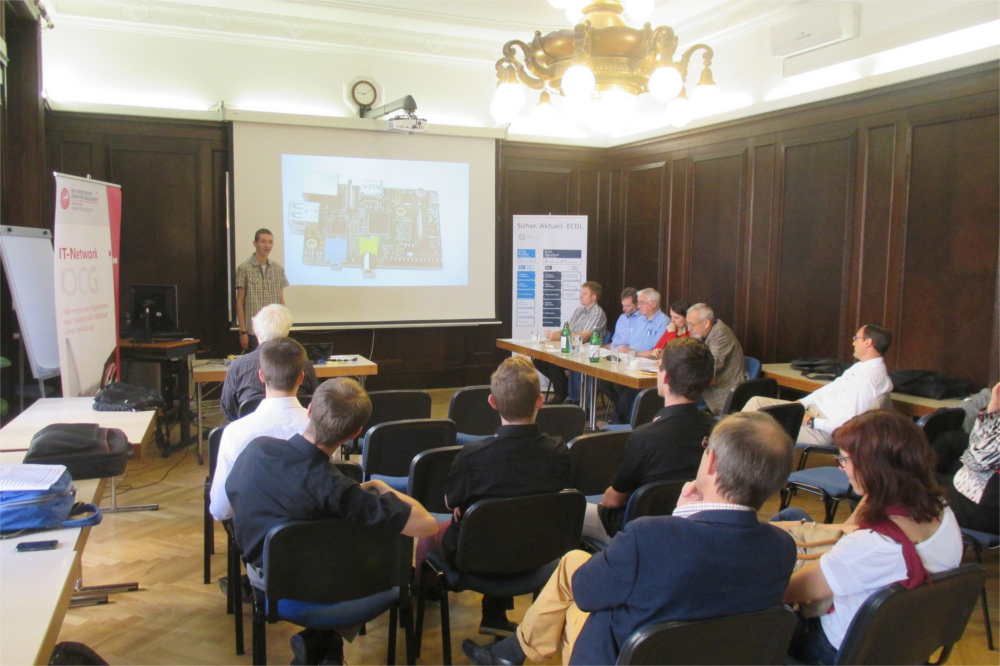
\includegraphics[width=\textwidth]{figures/ocg.jpg}
	\caption{Präsentation im Finale vom \textsf{computer creative wettbewerb}}
\end{figure}	


\includepdf[pages={1}]{figures/Urkunde.png}
